\section{Results}
\label{sec:results}

This section will describe all the experiments conducted to measure the effectiveness of kMatrix against existing streaming graph sketching techniques. 

We have considered CountMin, gSketch, TCM, gMatrix and kMatrix sketches in our experiments. These sketches can be categorized into two groups depending on the type of queries they are able to answer.

\begin{enumerate}
    \item \emph{Type I} - The sketches which support only the edge frequency queries, i.e. CountMin and gSketch.
    \item \emph{Type II} - The sketches which support many graph queries in general, i.e. TCM, gMatrix and kMatrix
\end{enumerate}

Since \emph{Type I} sketches cannot answer anything other than edge frequency queries, we have only included \emph{Type II} sketches in our comparisons against kMatrix.

\subsection{Build-time}

Here we investigated the time to add the entire dataset to the sketch. The sketches were allocated a constant memory size of 1 MB, and the number of hash functions was set to \(d = 7\). The edges were streamed at the maximum throughput of each sketch. Therefore this experiment gives an idea about the average insertion rate of edges for each sketch. A minor drawback of kMatrix is that it takes some time for its initialization stage. However, this initialization time becomes negligible compared to the advantage that kMatrix receives over time due to its faster streaming rate. In both Fig.~\ref{fig:btt-a} and Fig.~\ref{fig:btt-c}, it has managed to outperform other sketching techniques by a significant margin. In Fig.~\ref{fig:btt-b}, kMatrix has shown comparable performance to gMatrix. With the increase of the data contained within the sketch, the number of hash collisions in TCM and gMatrix has grown over time, increasing the computational cost of inserting a new edge. kMatrix has maintained a relatively lower build time as a result of its lower number of hash collisions due to the sketch partitioning before inserting the edges.

\begin{figure}[htbp] 
    \centering
    \subfloat[unicorn-wget\label{fig:btt-a}]{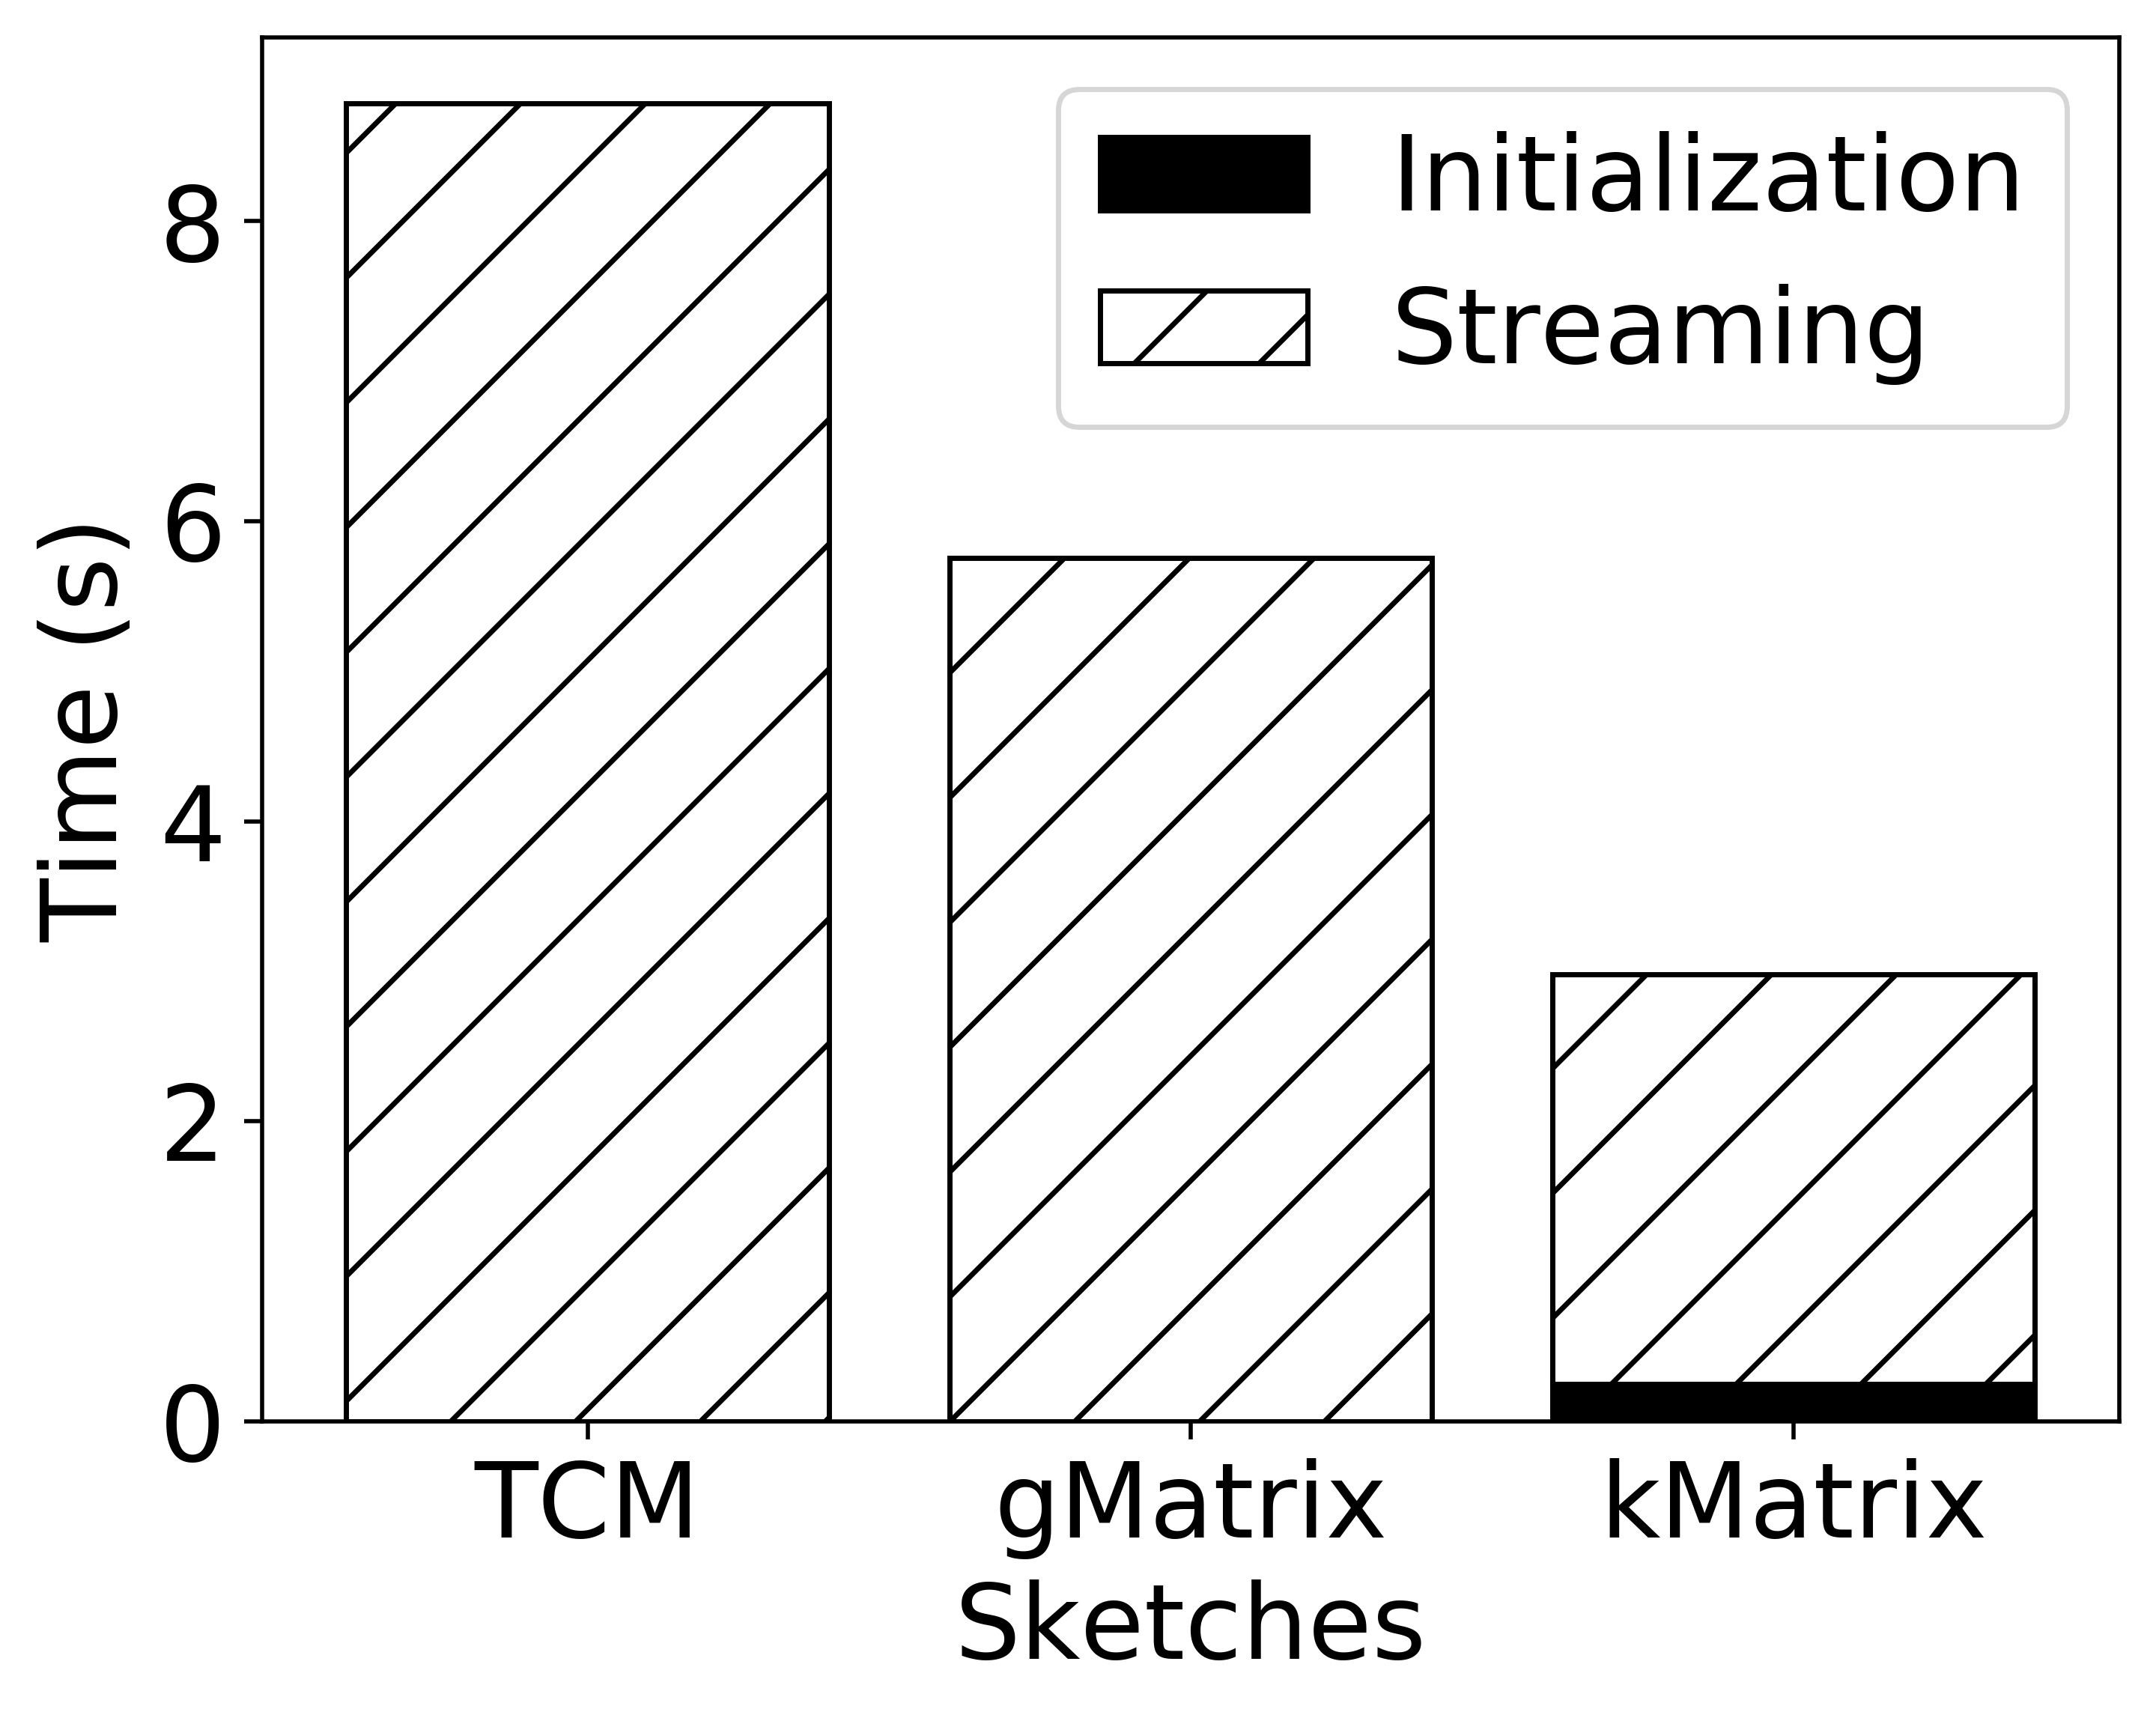
\includegraphics[width=0.45\linewidth]{img/buildtime_1024_unicorn-wget.png}}
    \hfill
    \subfloat[email-EuAll\label{fig:btt-b}]{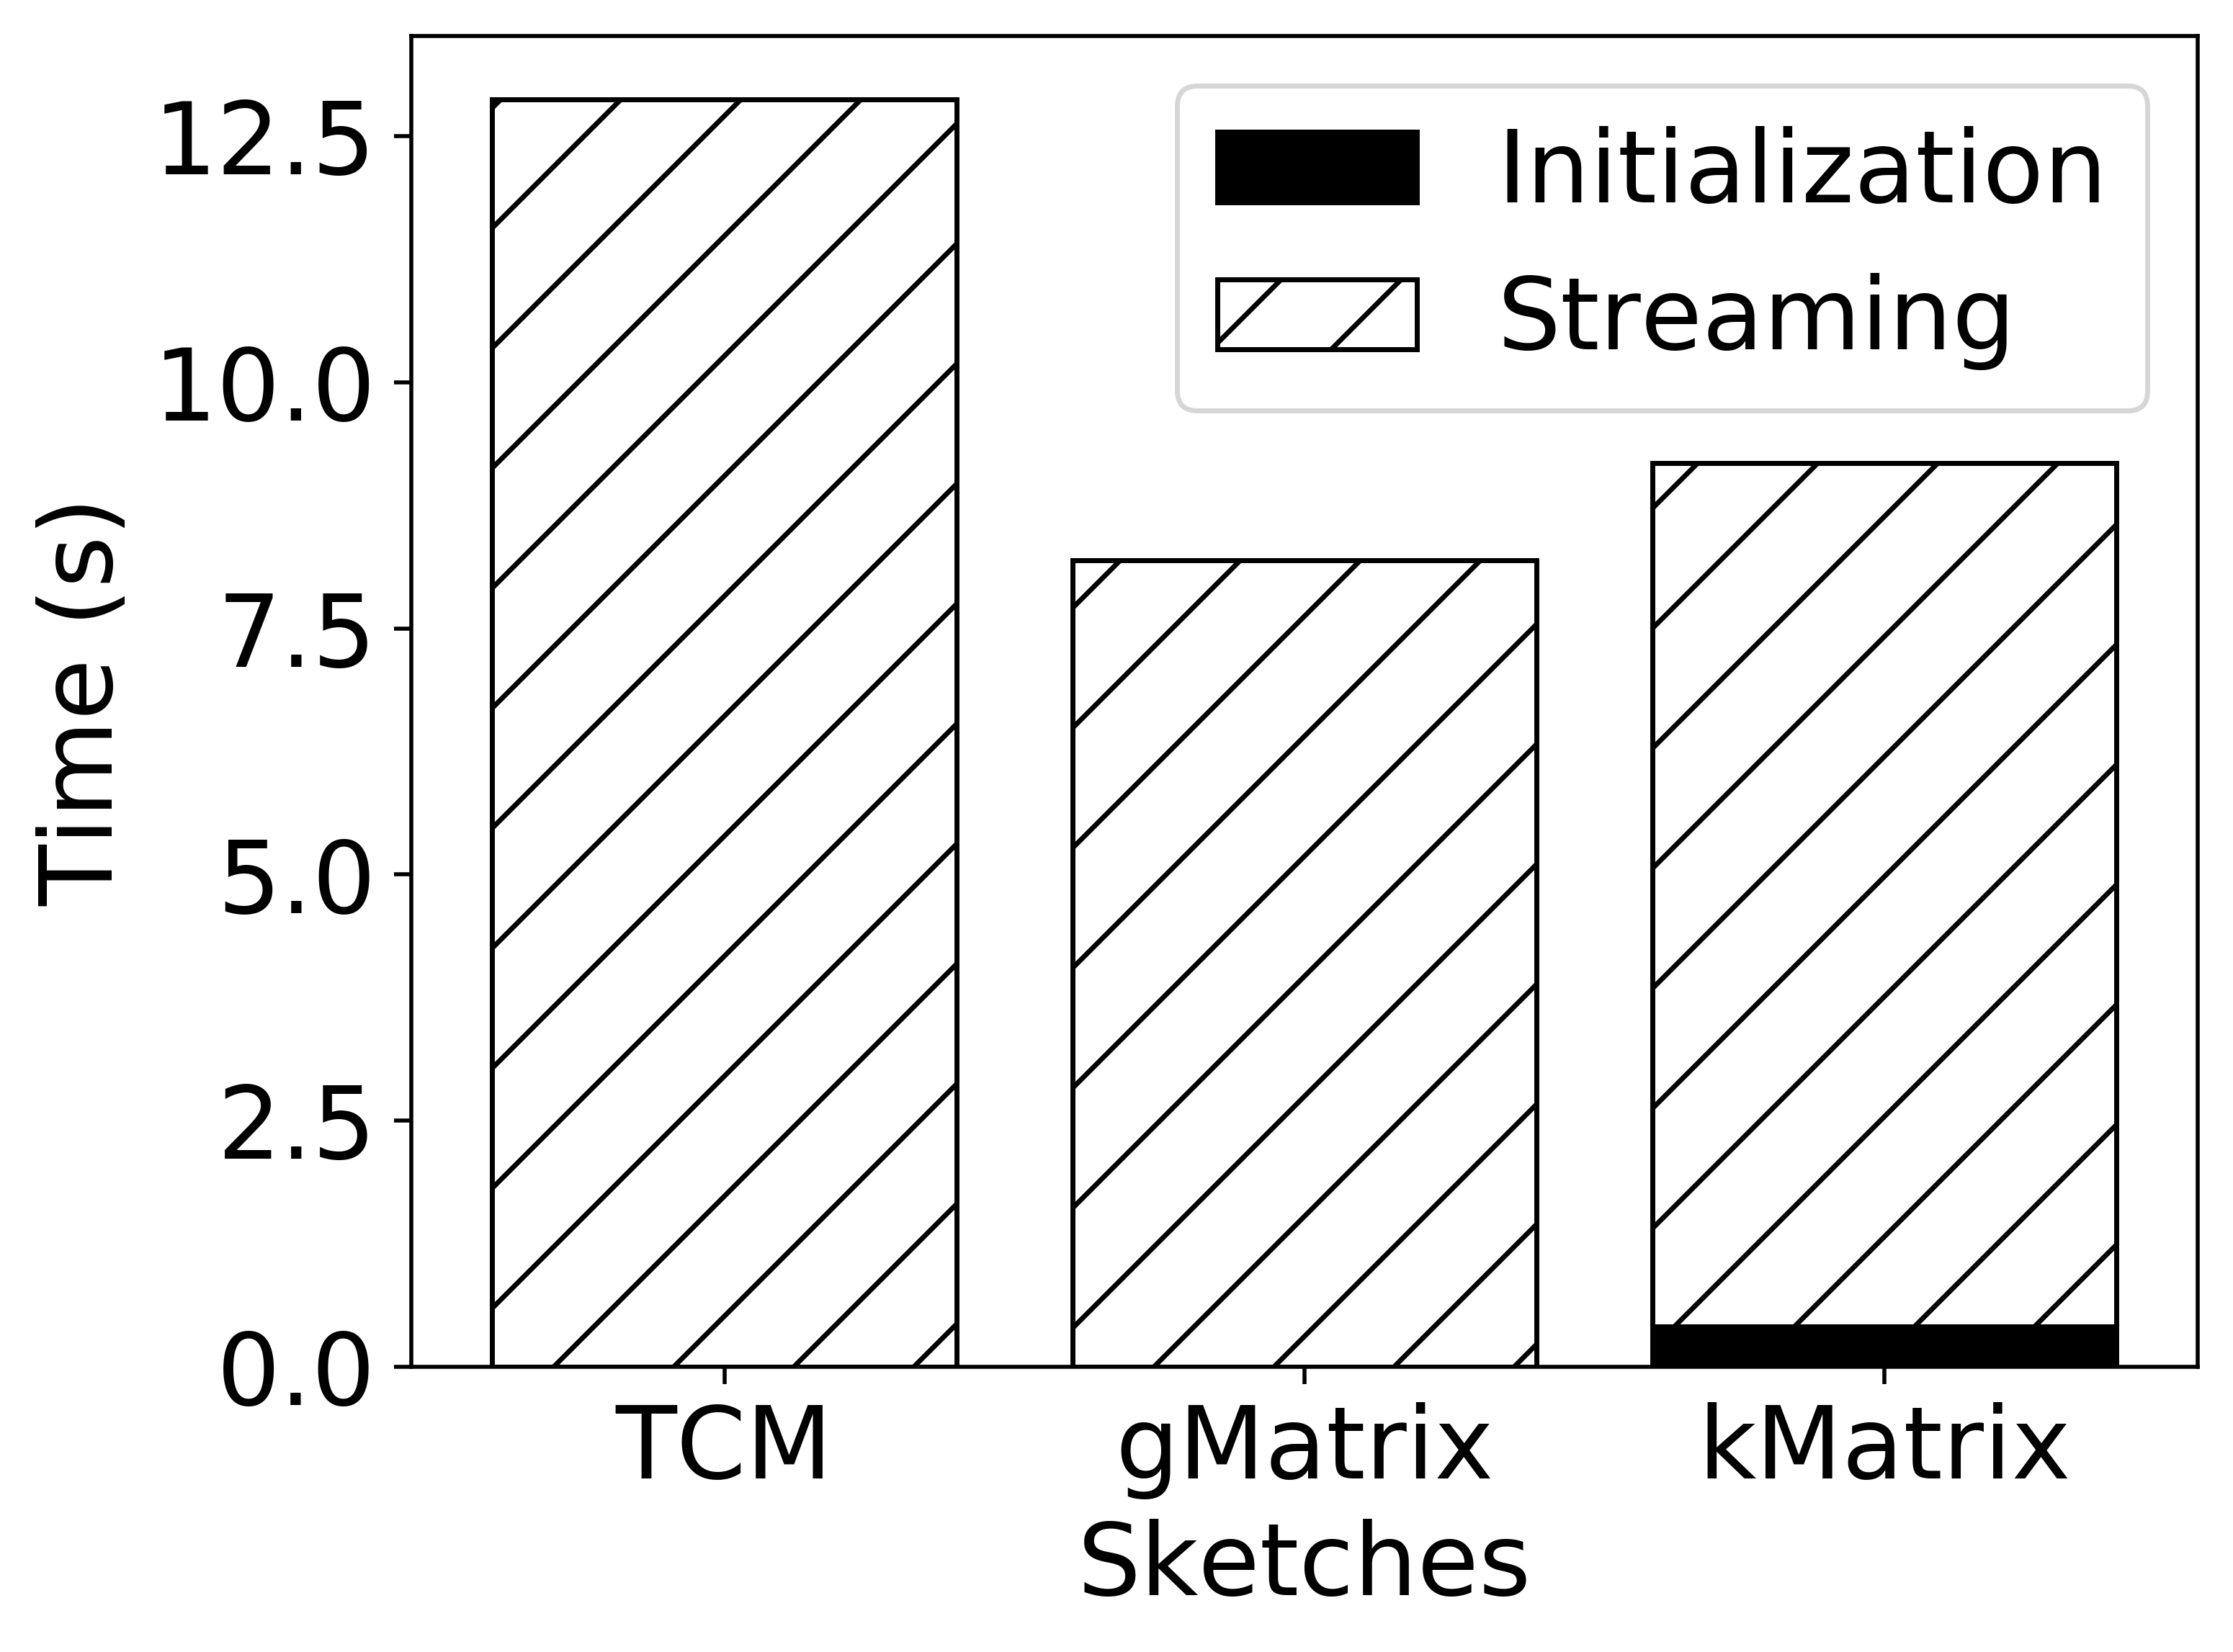
\includegraphics[width=0.45\linewidth]{img/buildtime_1024_email-EuAll.png}}
    \hfill
    \subfloat[cit-HepPh\label{fig:btt-c}]{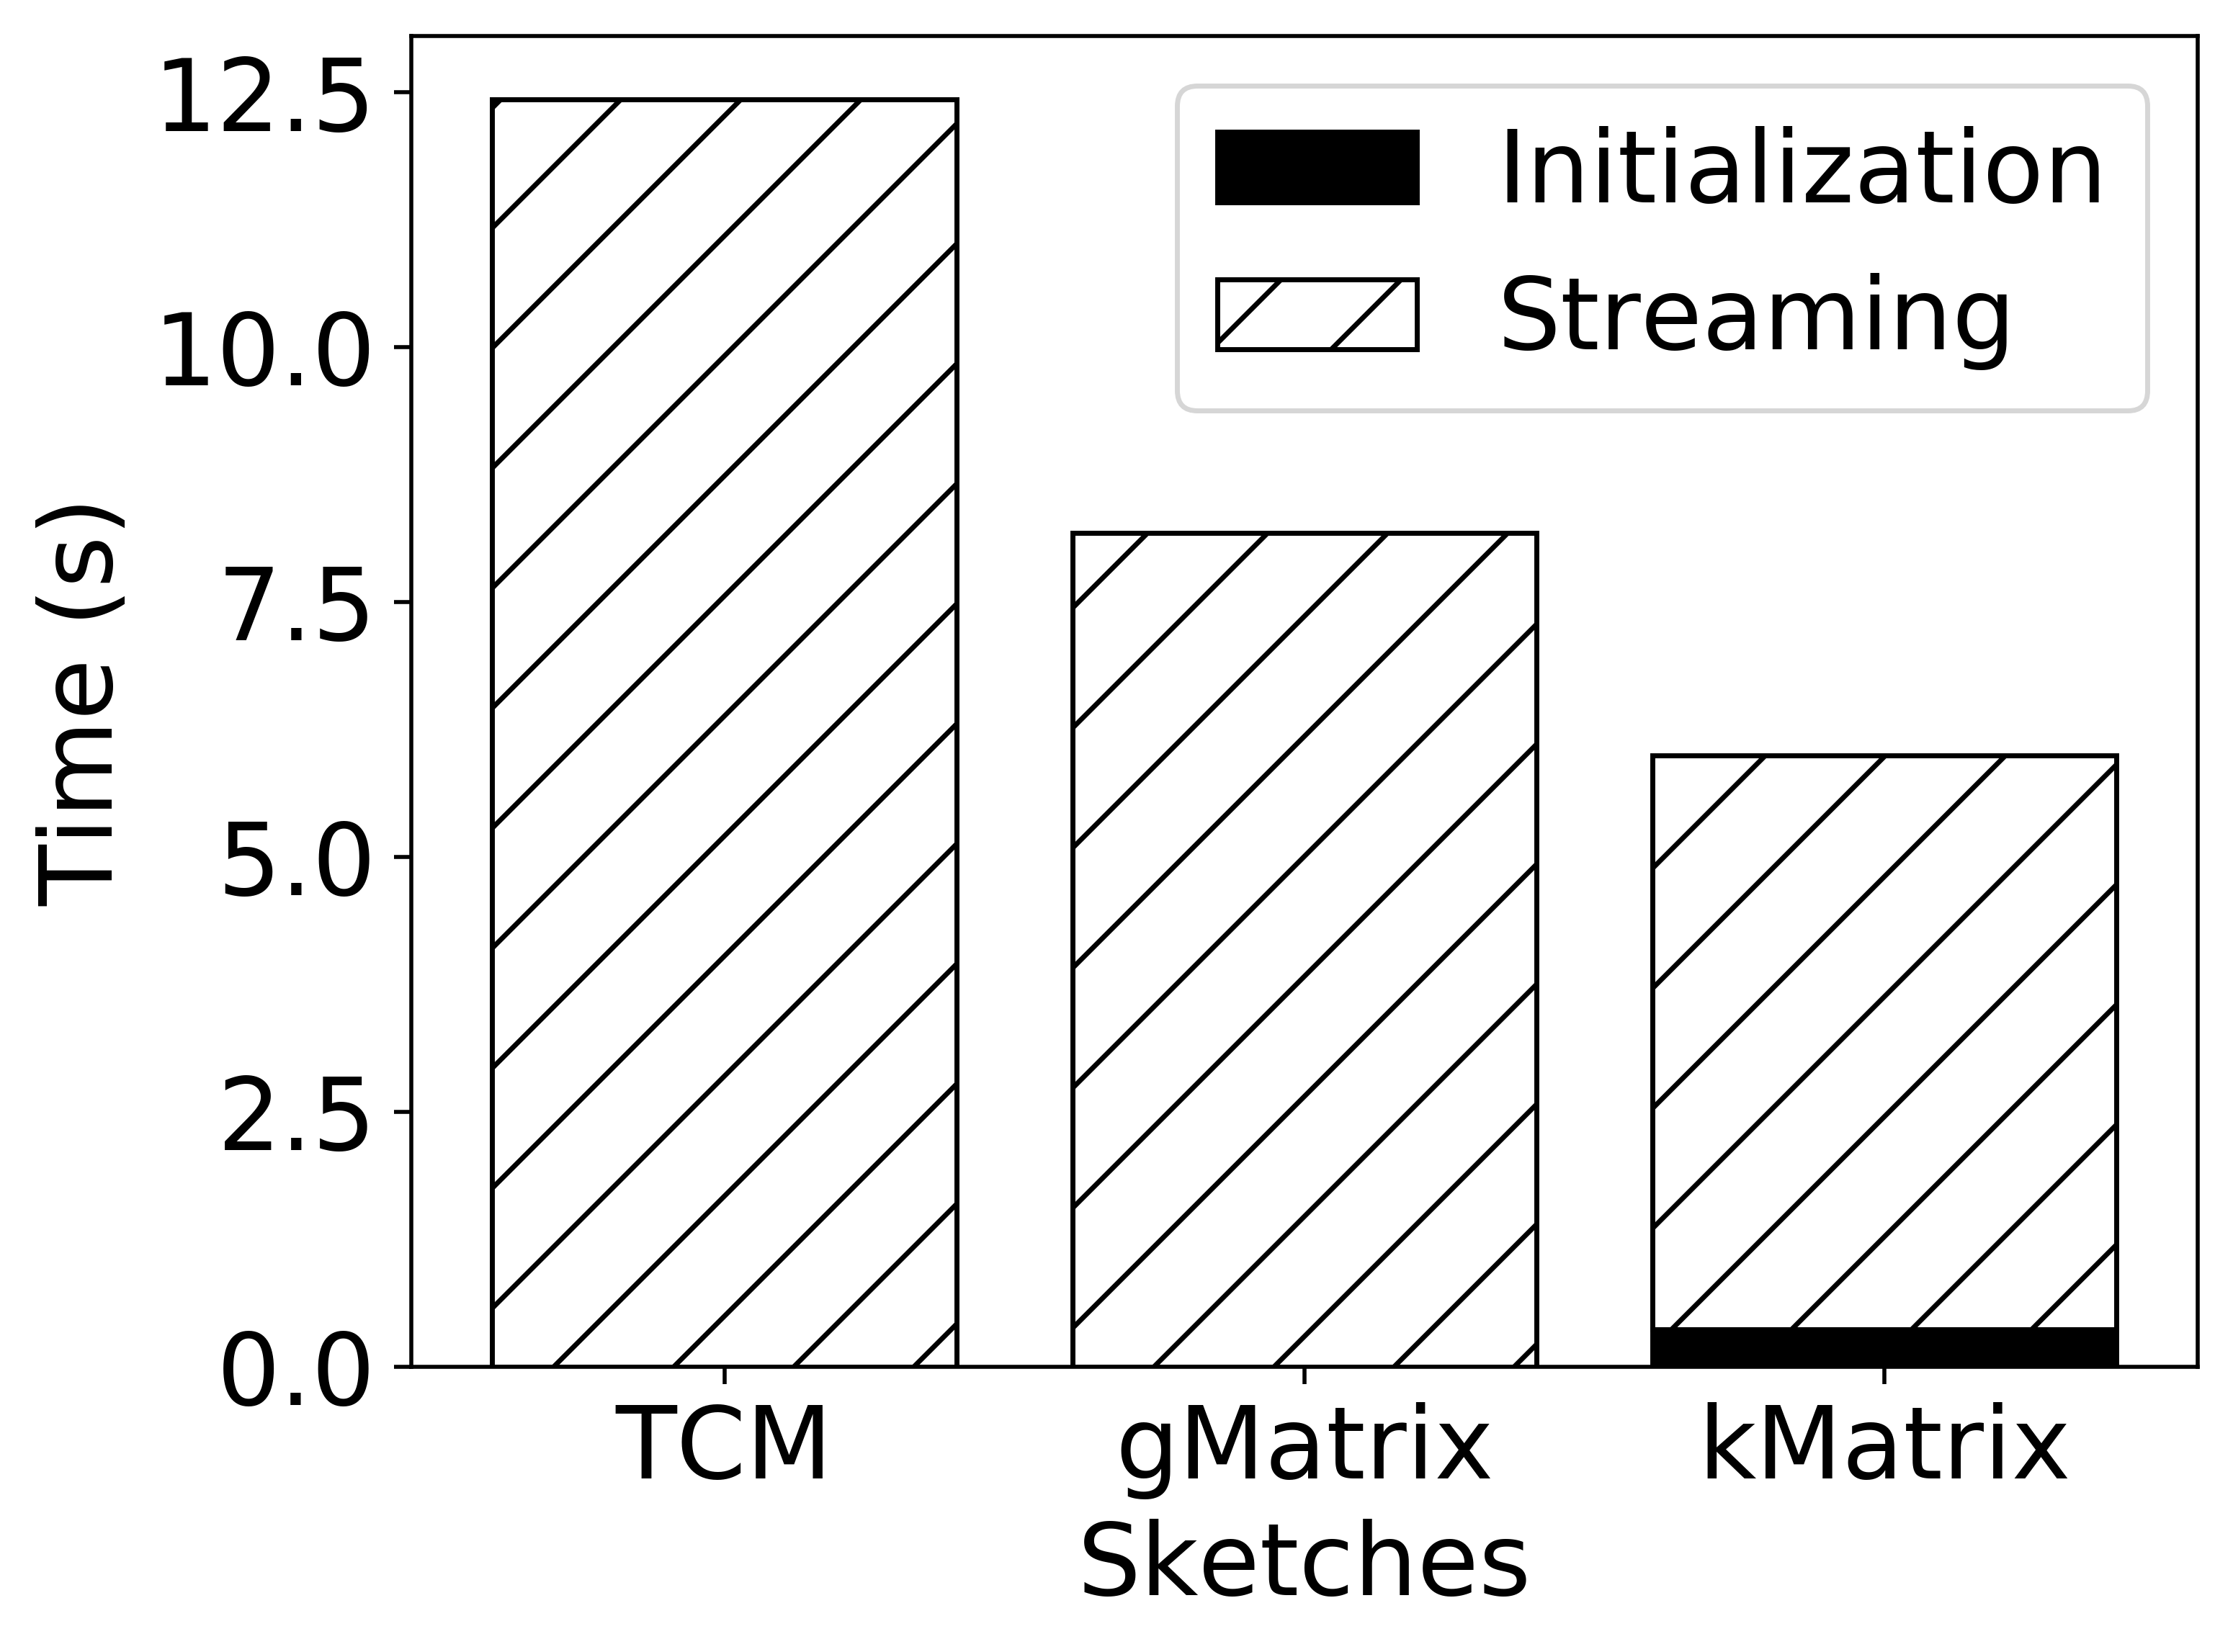
\includegraphics[width=0.45\linewidth]{img/buildtime_1024_cit-HepPh.png}}
    \caption{Build-time}
    \label{fig:buildtime-test}
\end{figure}

\subsection{Edge queries}

This experiment investigates how accurately the kMatrix can answer the edge queries after the summarization process. For this, we let our datastream get summarized into the sketch and then queried the frequency of different edges chosen at random. The experiment was repeated for each sketch for the sizes, 200 KB, 300 KB, 400 KB and 512 KB while keeping the number of hash functions at \(d = 7\). We have used average relative error and the number of effective queries as the evaluation matrices for this experiment.

\subsubsection{Average Relative Error}
\label{section:results_are}

\begin{figure}[htbp] 
    \centering
    \subfloat[unicorn-wget\label{fig:are-a}]{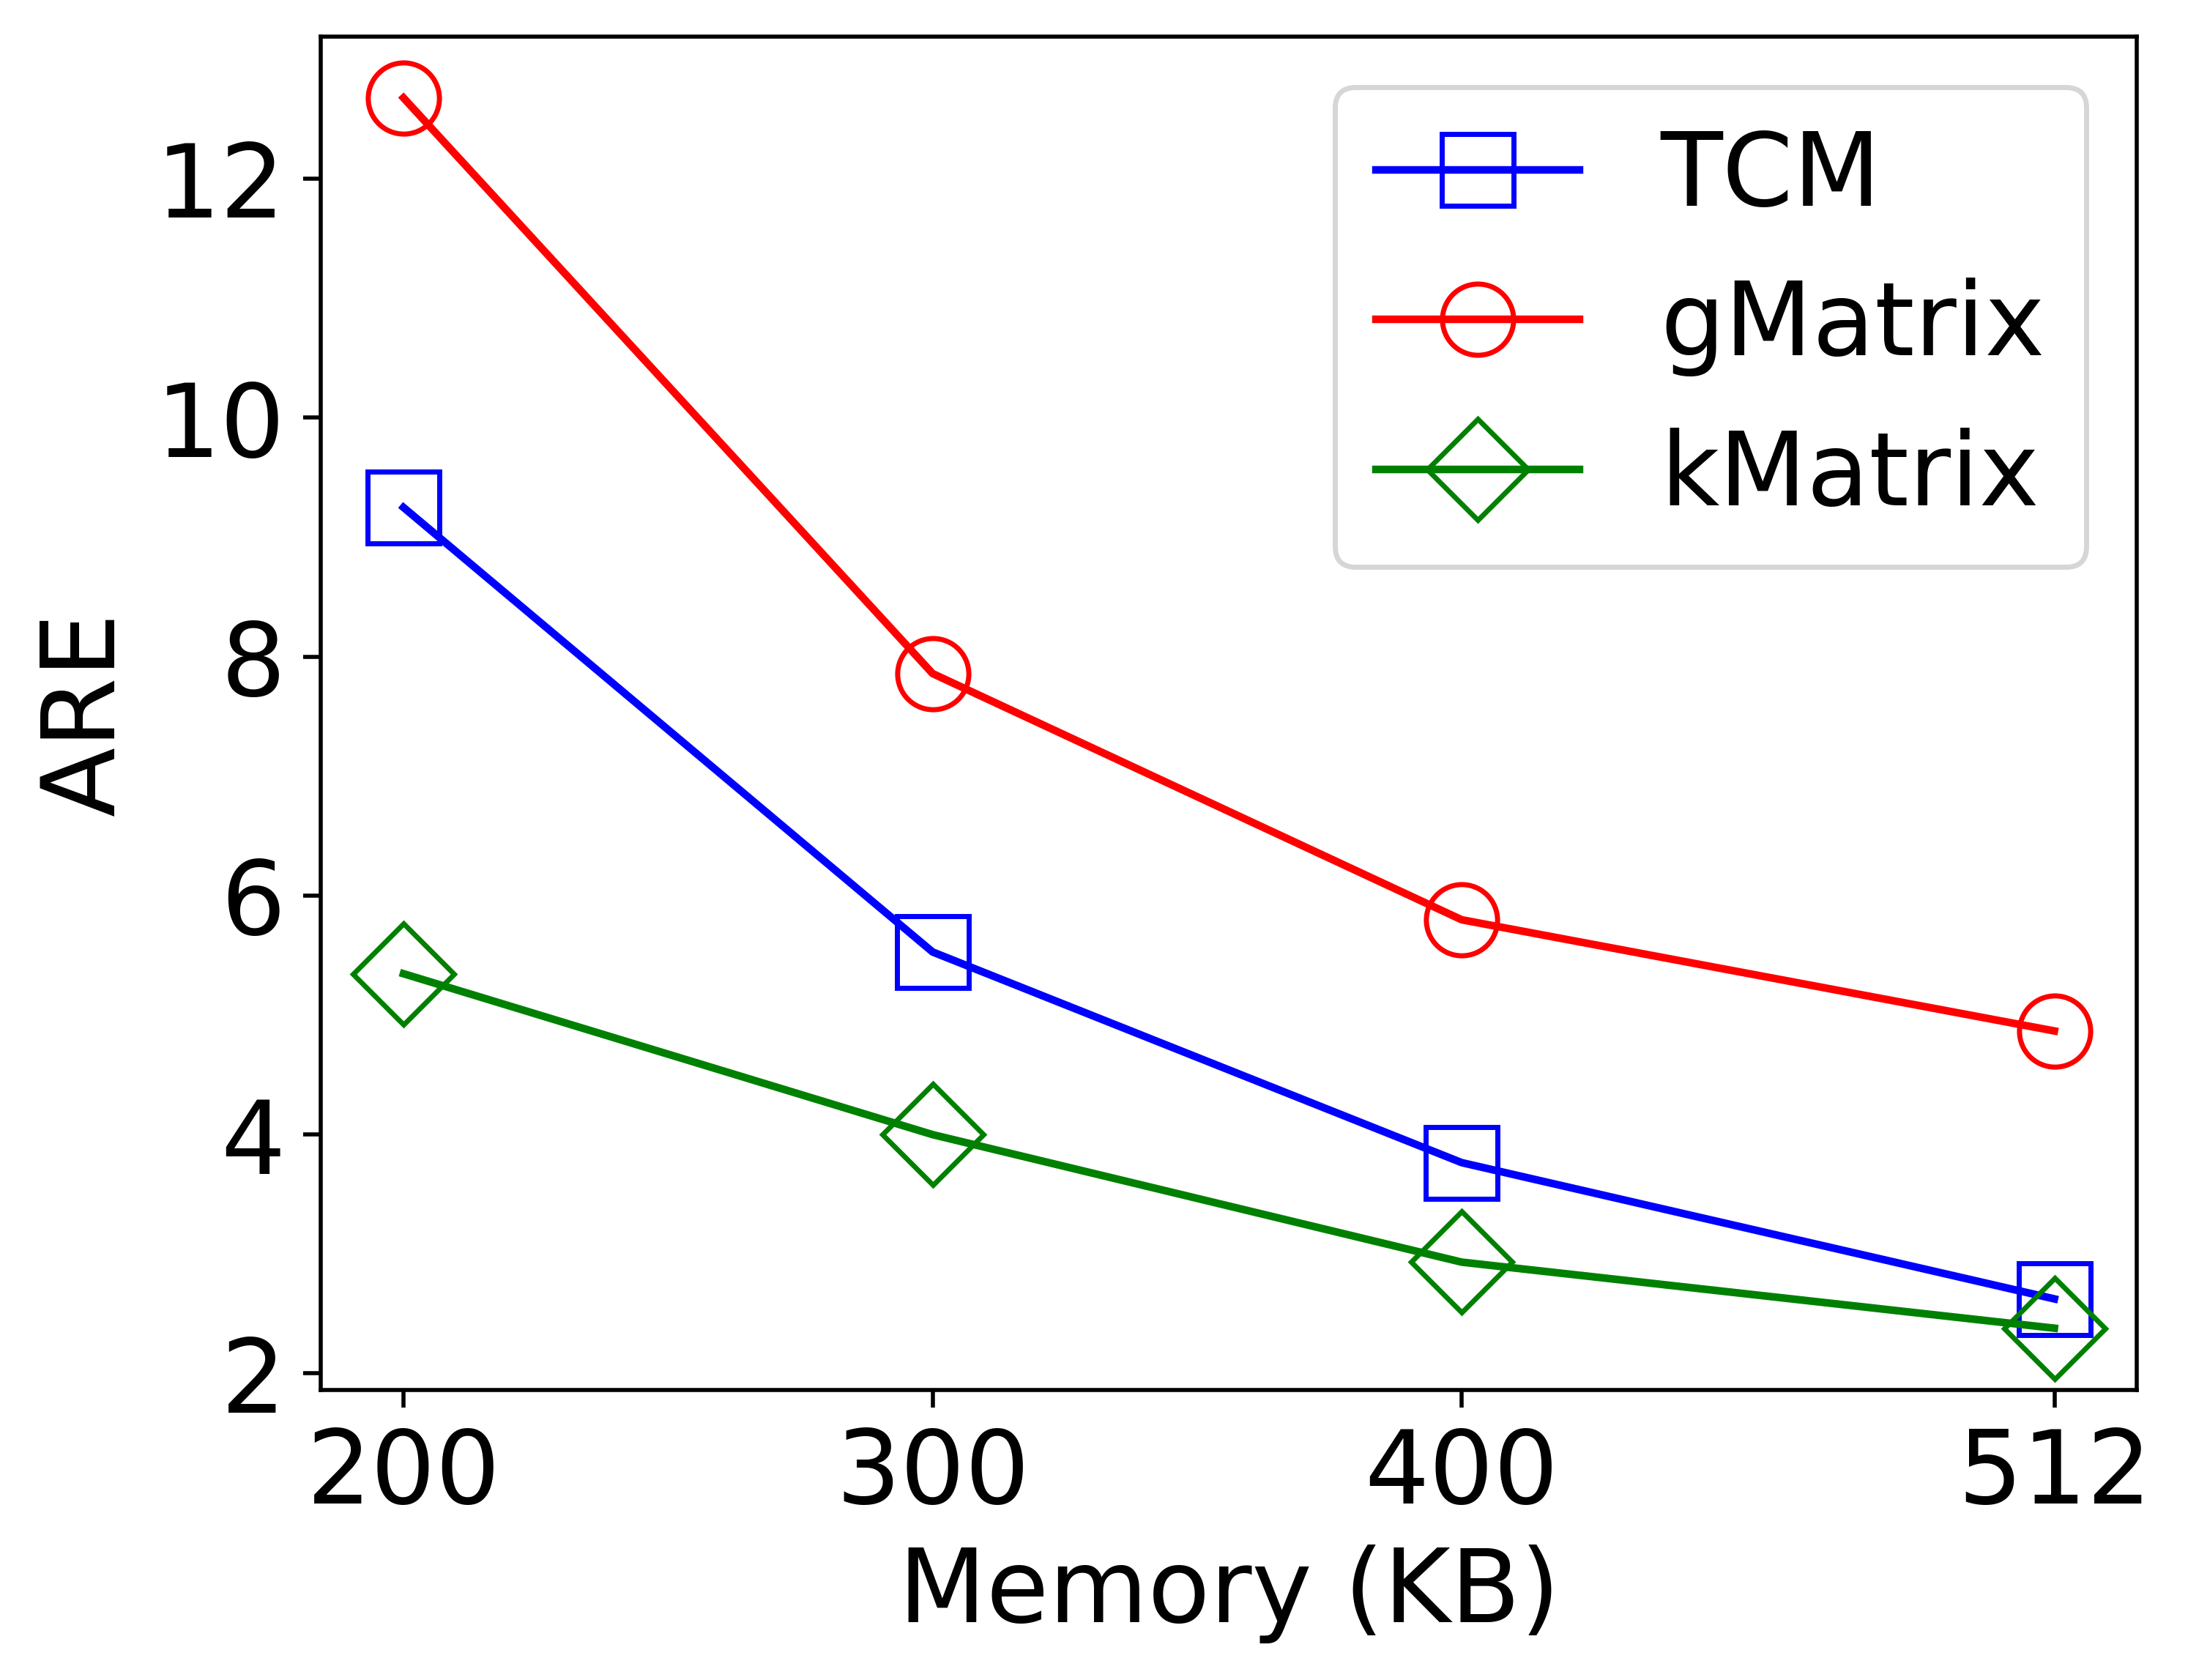
\includegraphics[width=0.45\linewidth]{img/edge_query_are_unicorn-wget.png}}
    \hfill
    \subfloat[email-EuAll\label{fig:are-b}]{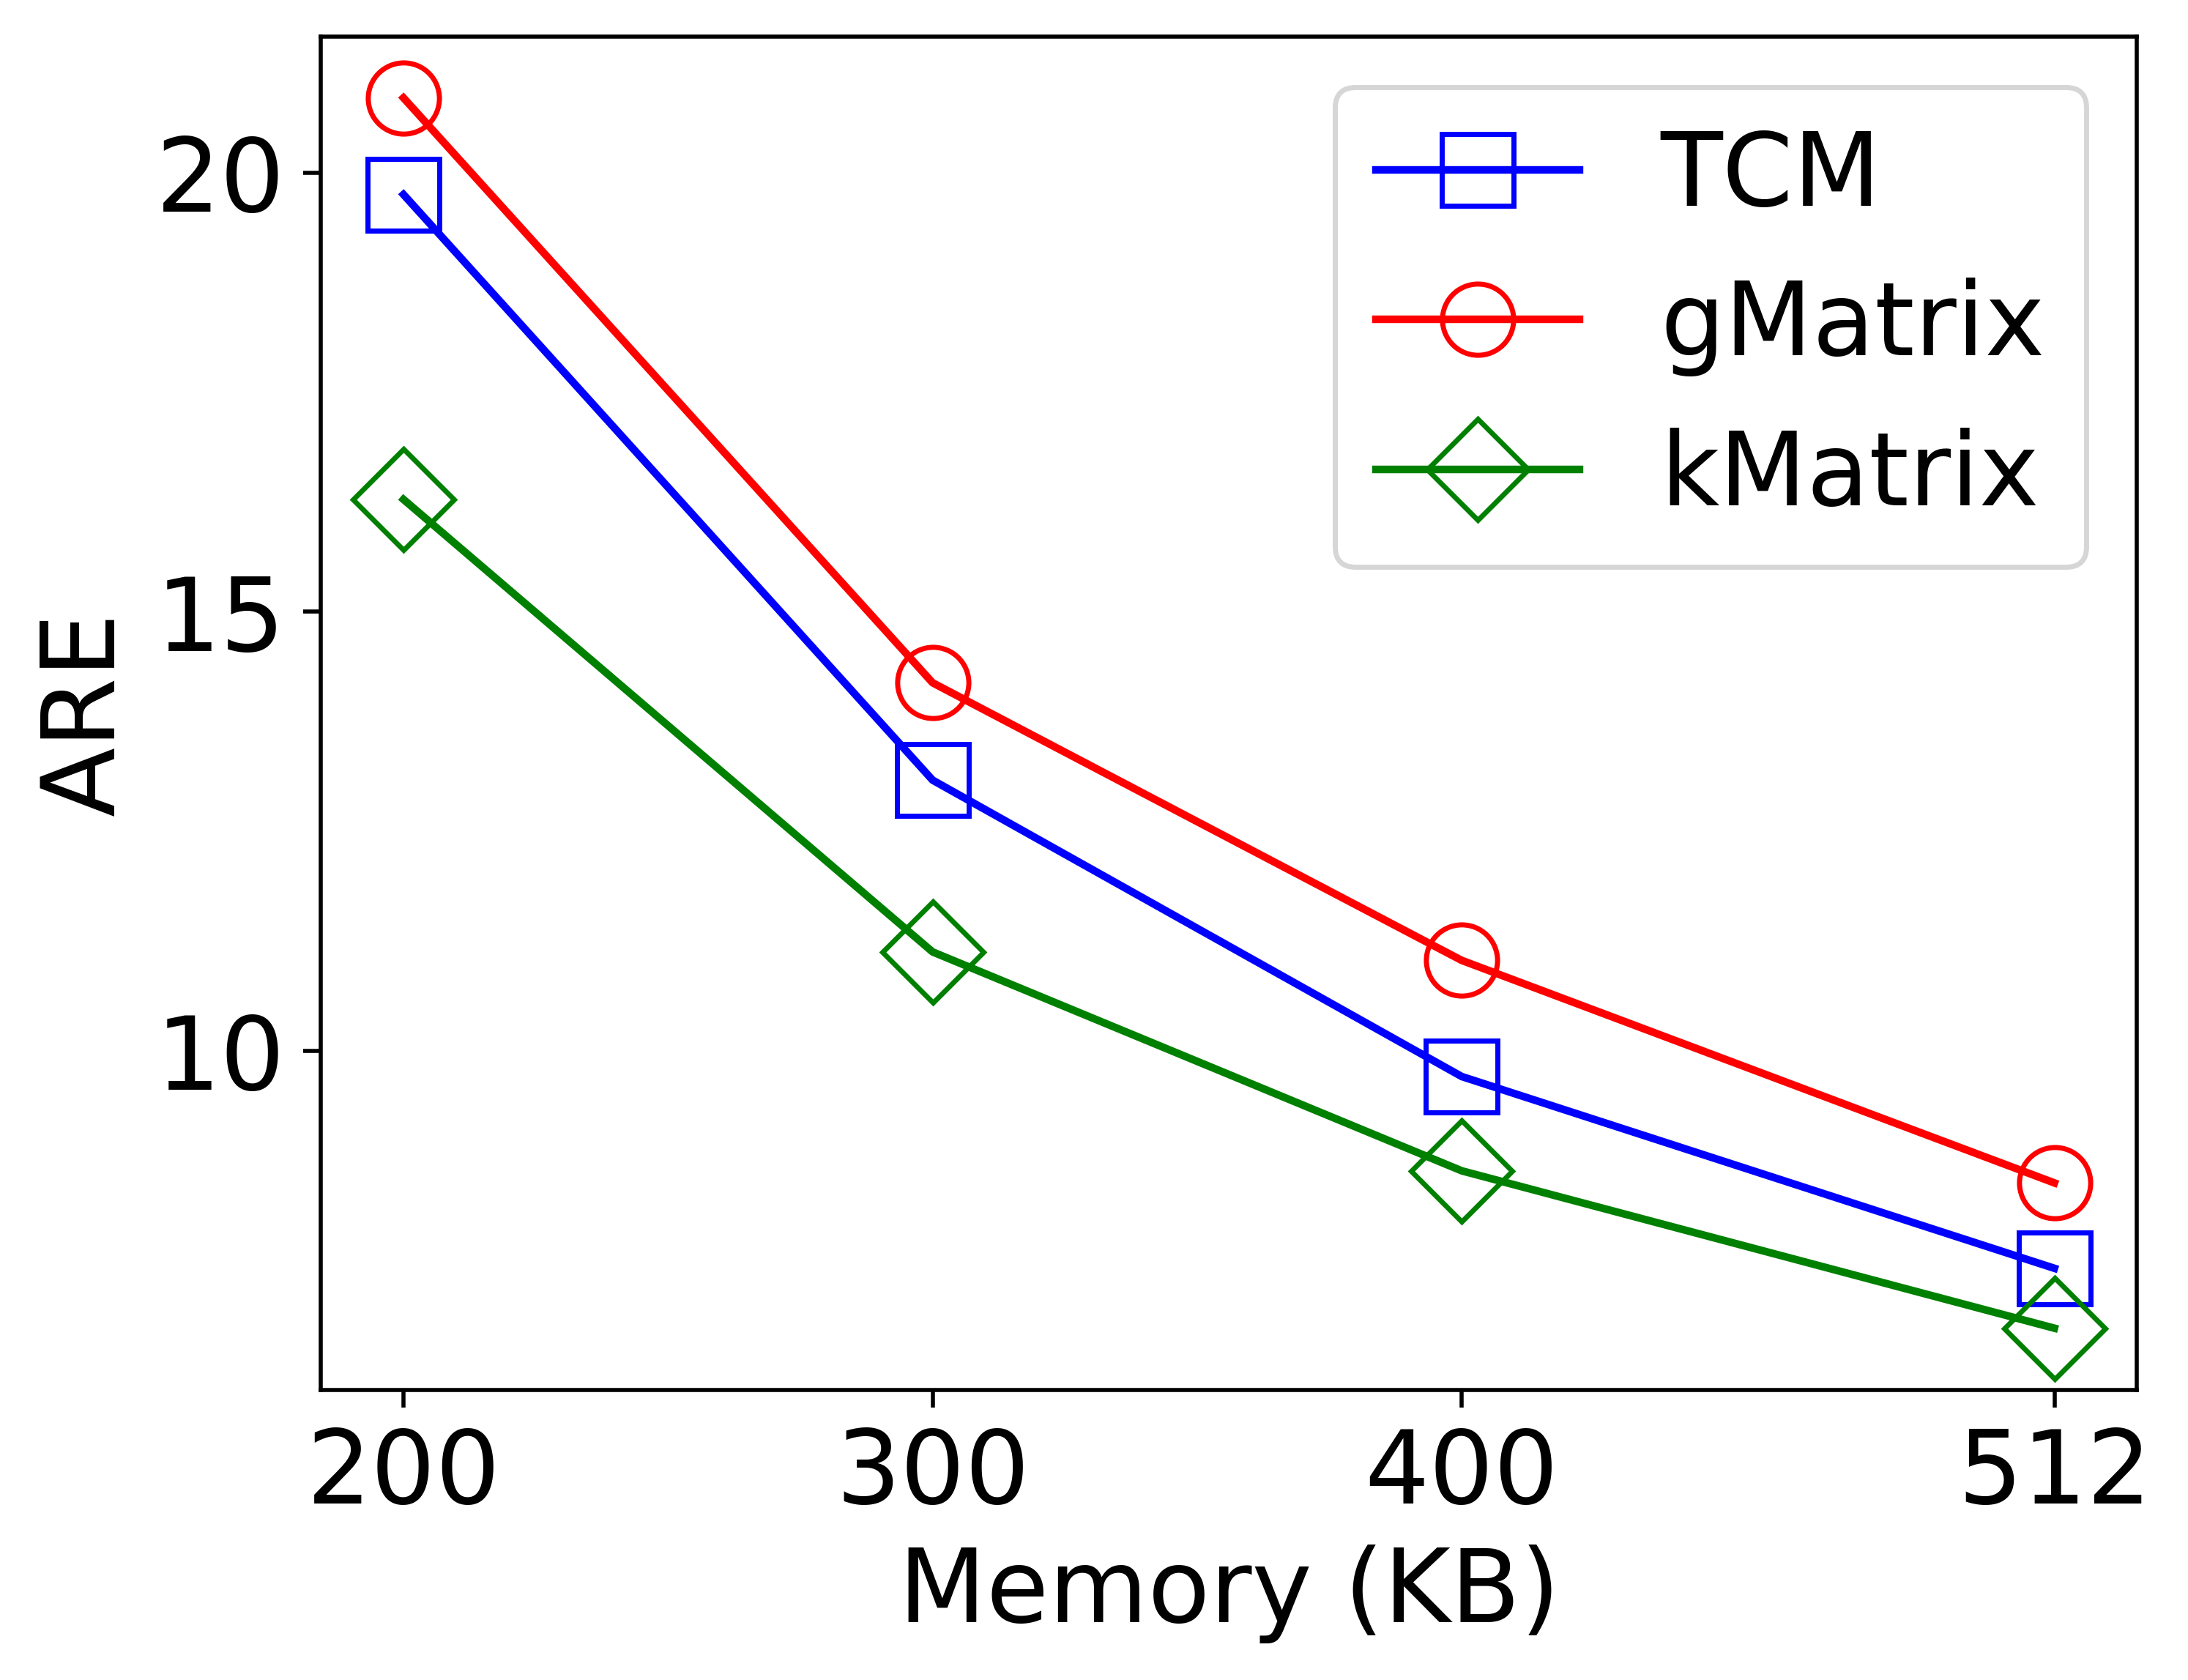
\includegraphics[width=0.45\linewidth]{img/edge_query_are_email-EuAll.png}}
    \hfill
    \subfloat[cit-HepPh\label{fig:are-c}]{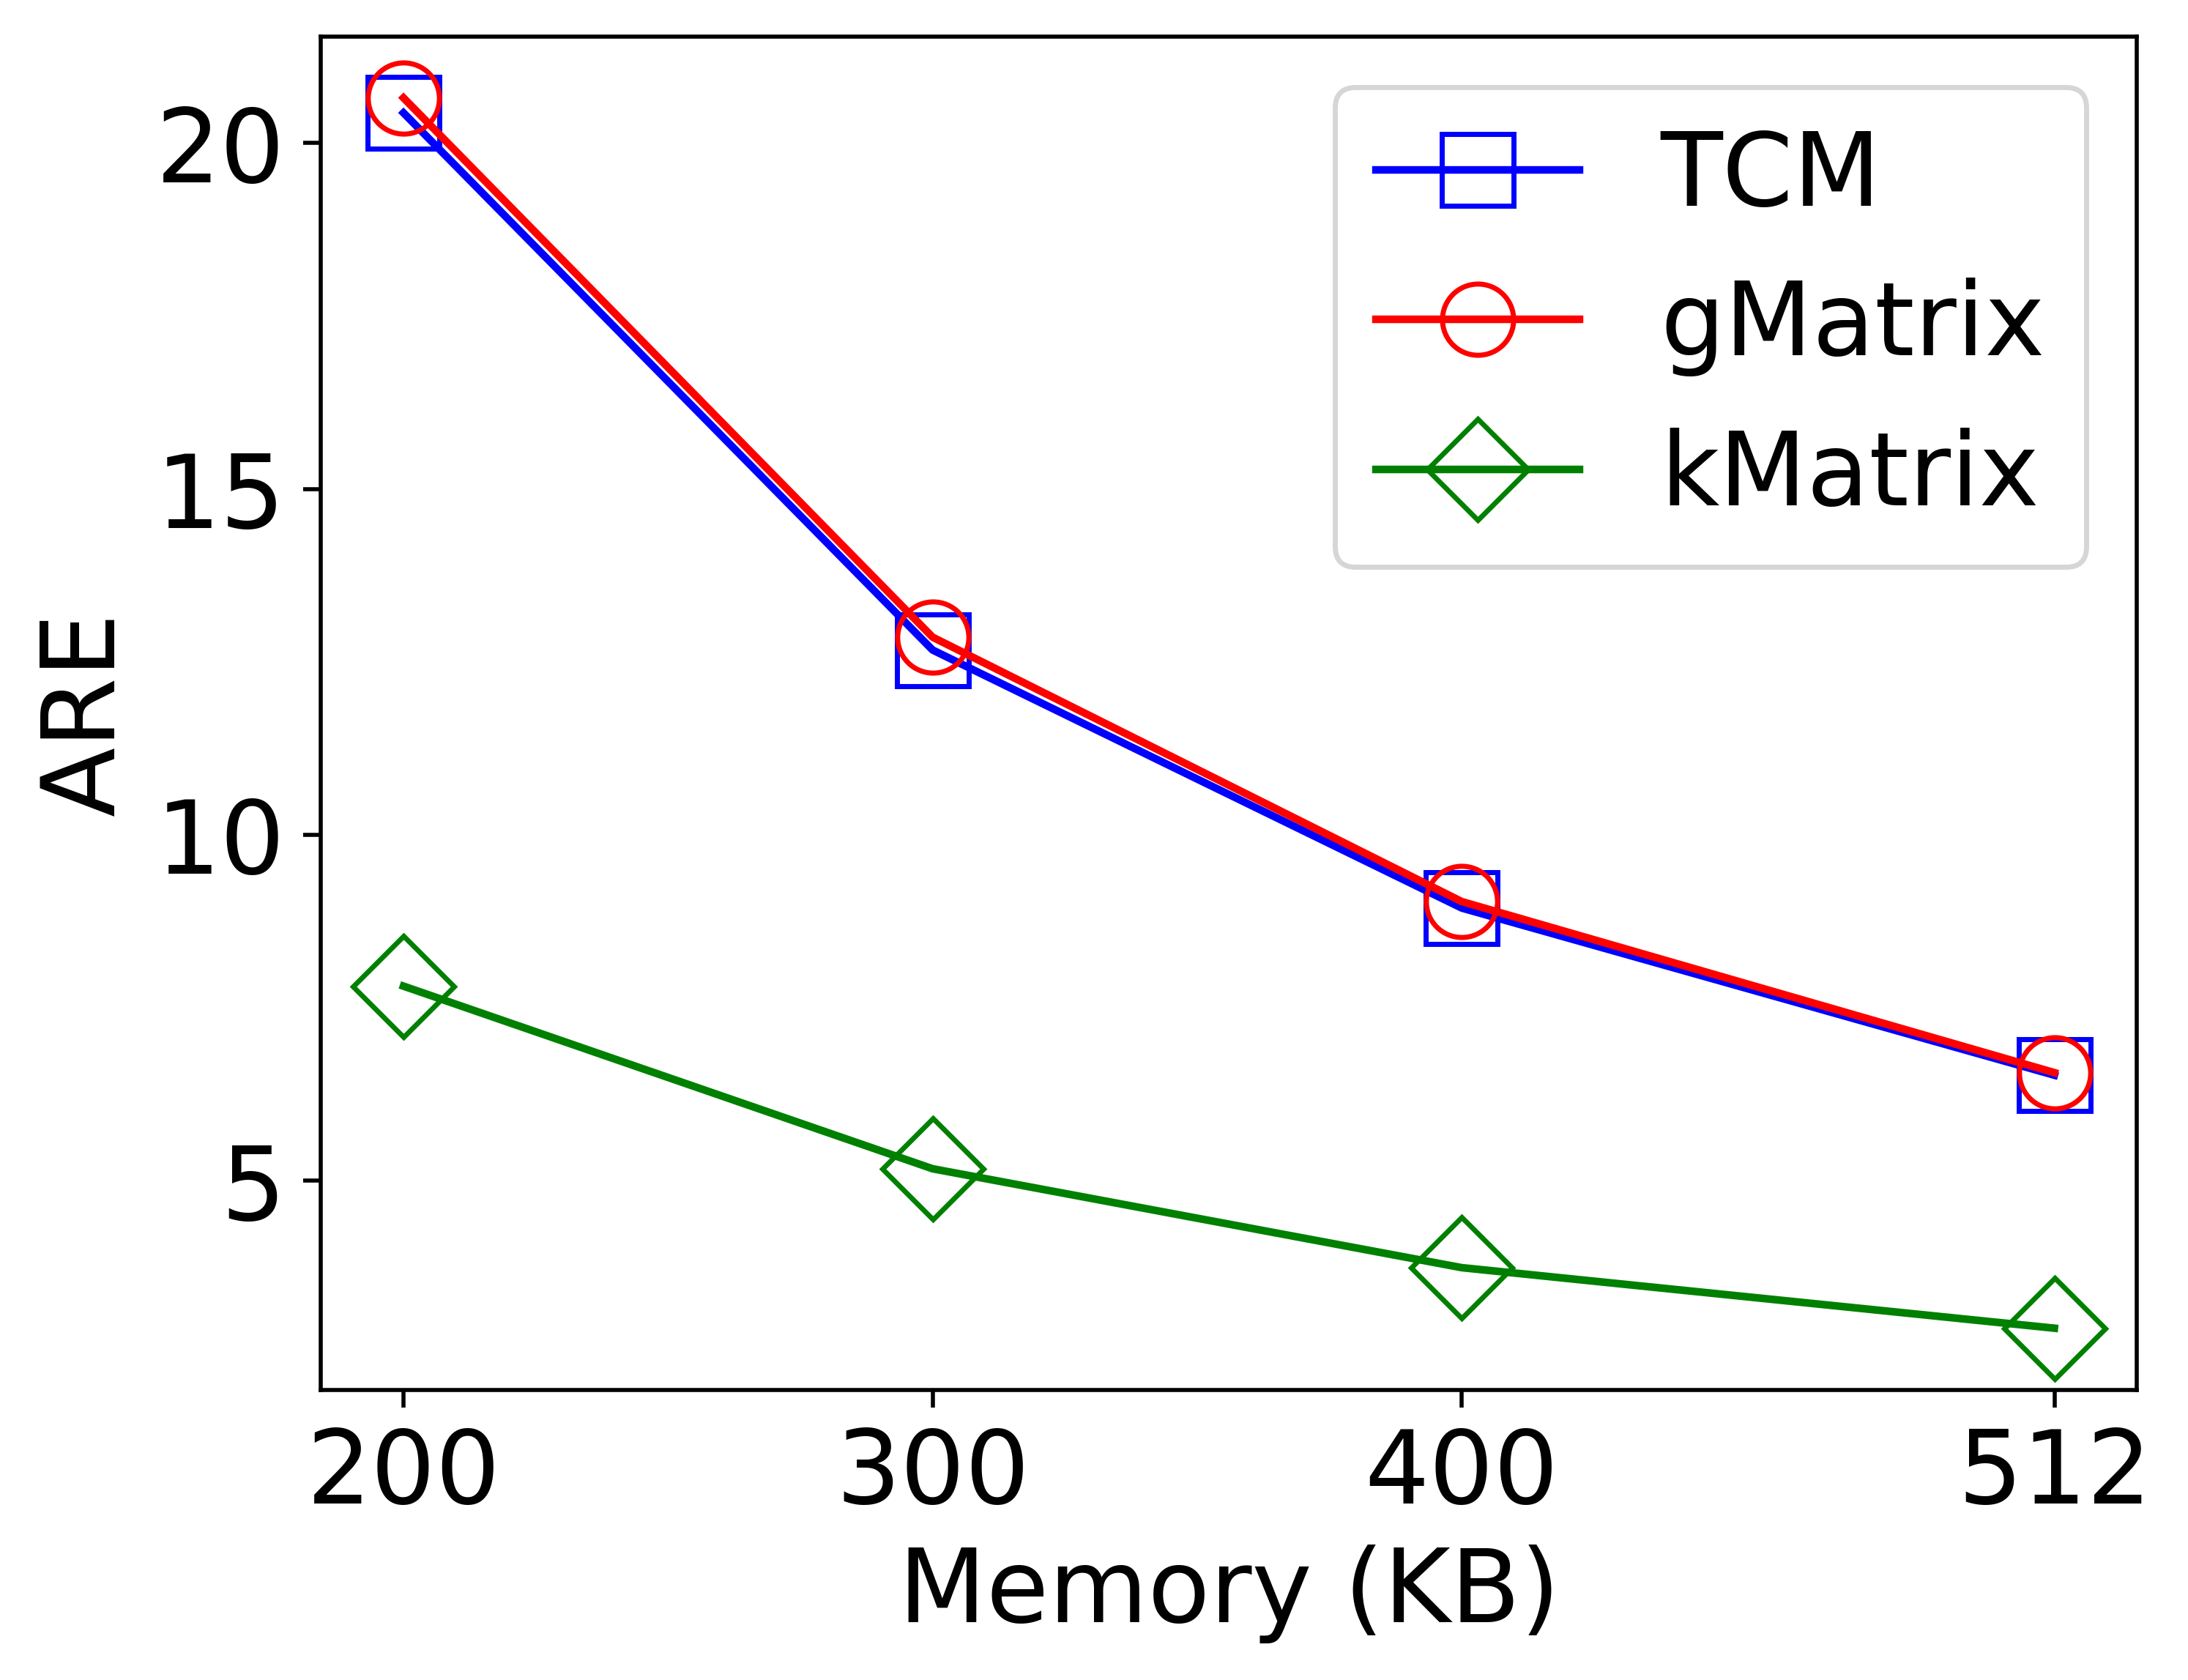
\includegraphics[width=0.45\linewidth]{img/edge_query_are_cit-HepPh.png}}
    \caption{Average relative error}
    \label{fig:edgq-queries-are-test}
\end{figure}

kMatrix showed significantly low ARE than all the other sketches for the three datasets we chose. The reason is that kMatrix can maintain frequency uniformity within each partition, making kMatrix relatively more immune to hash collisions than TCM and gMatrix. It is clear from the experimental evidence shown in Fig.~\ref{fig:edgq-queries-are-test} that kMatrix vastly outperforms the other state of the art sketching techniques. The superiority of our solution is more apparent when the allocated memory is low.

\subsubsection{Number of Effective Queries}

\begin{figure}[htbp] 
    \centering
    \subfloat[unicorn-wget\label{fig:neq-a}]{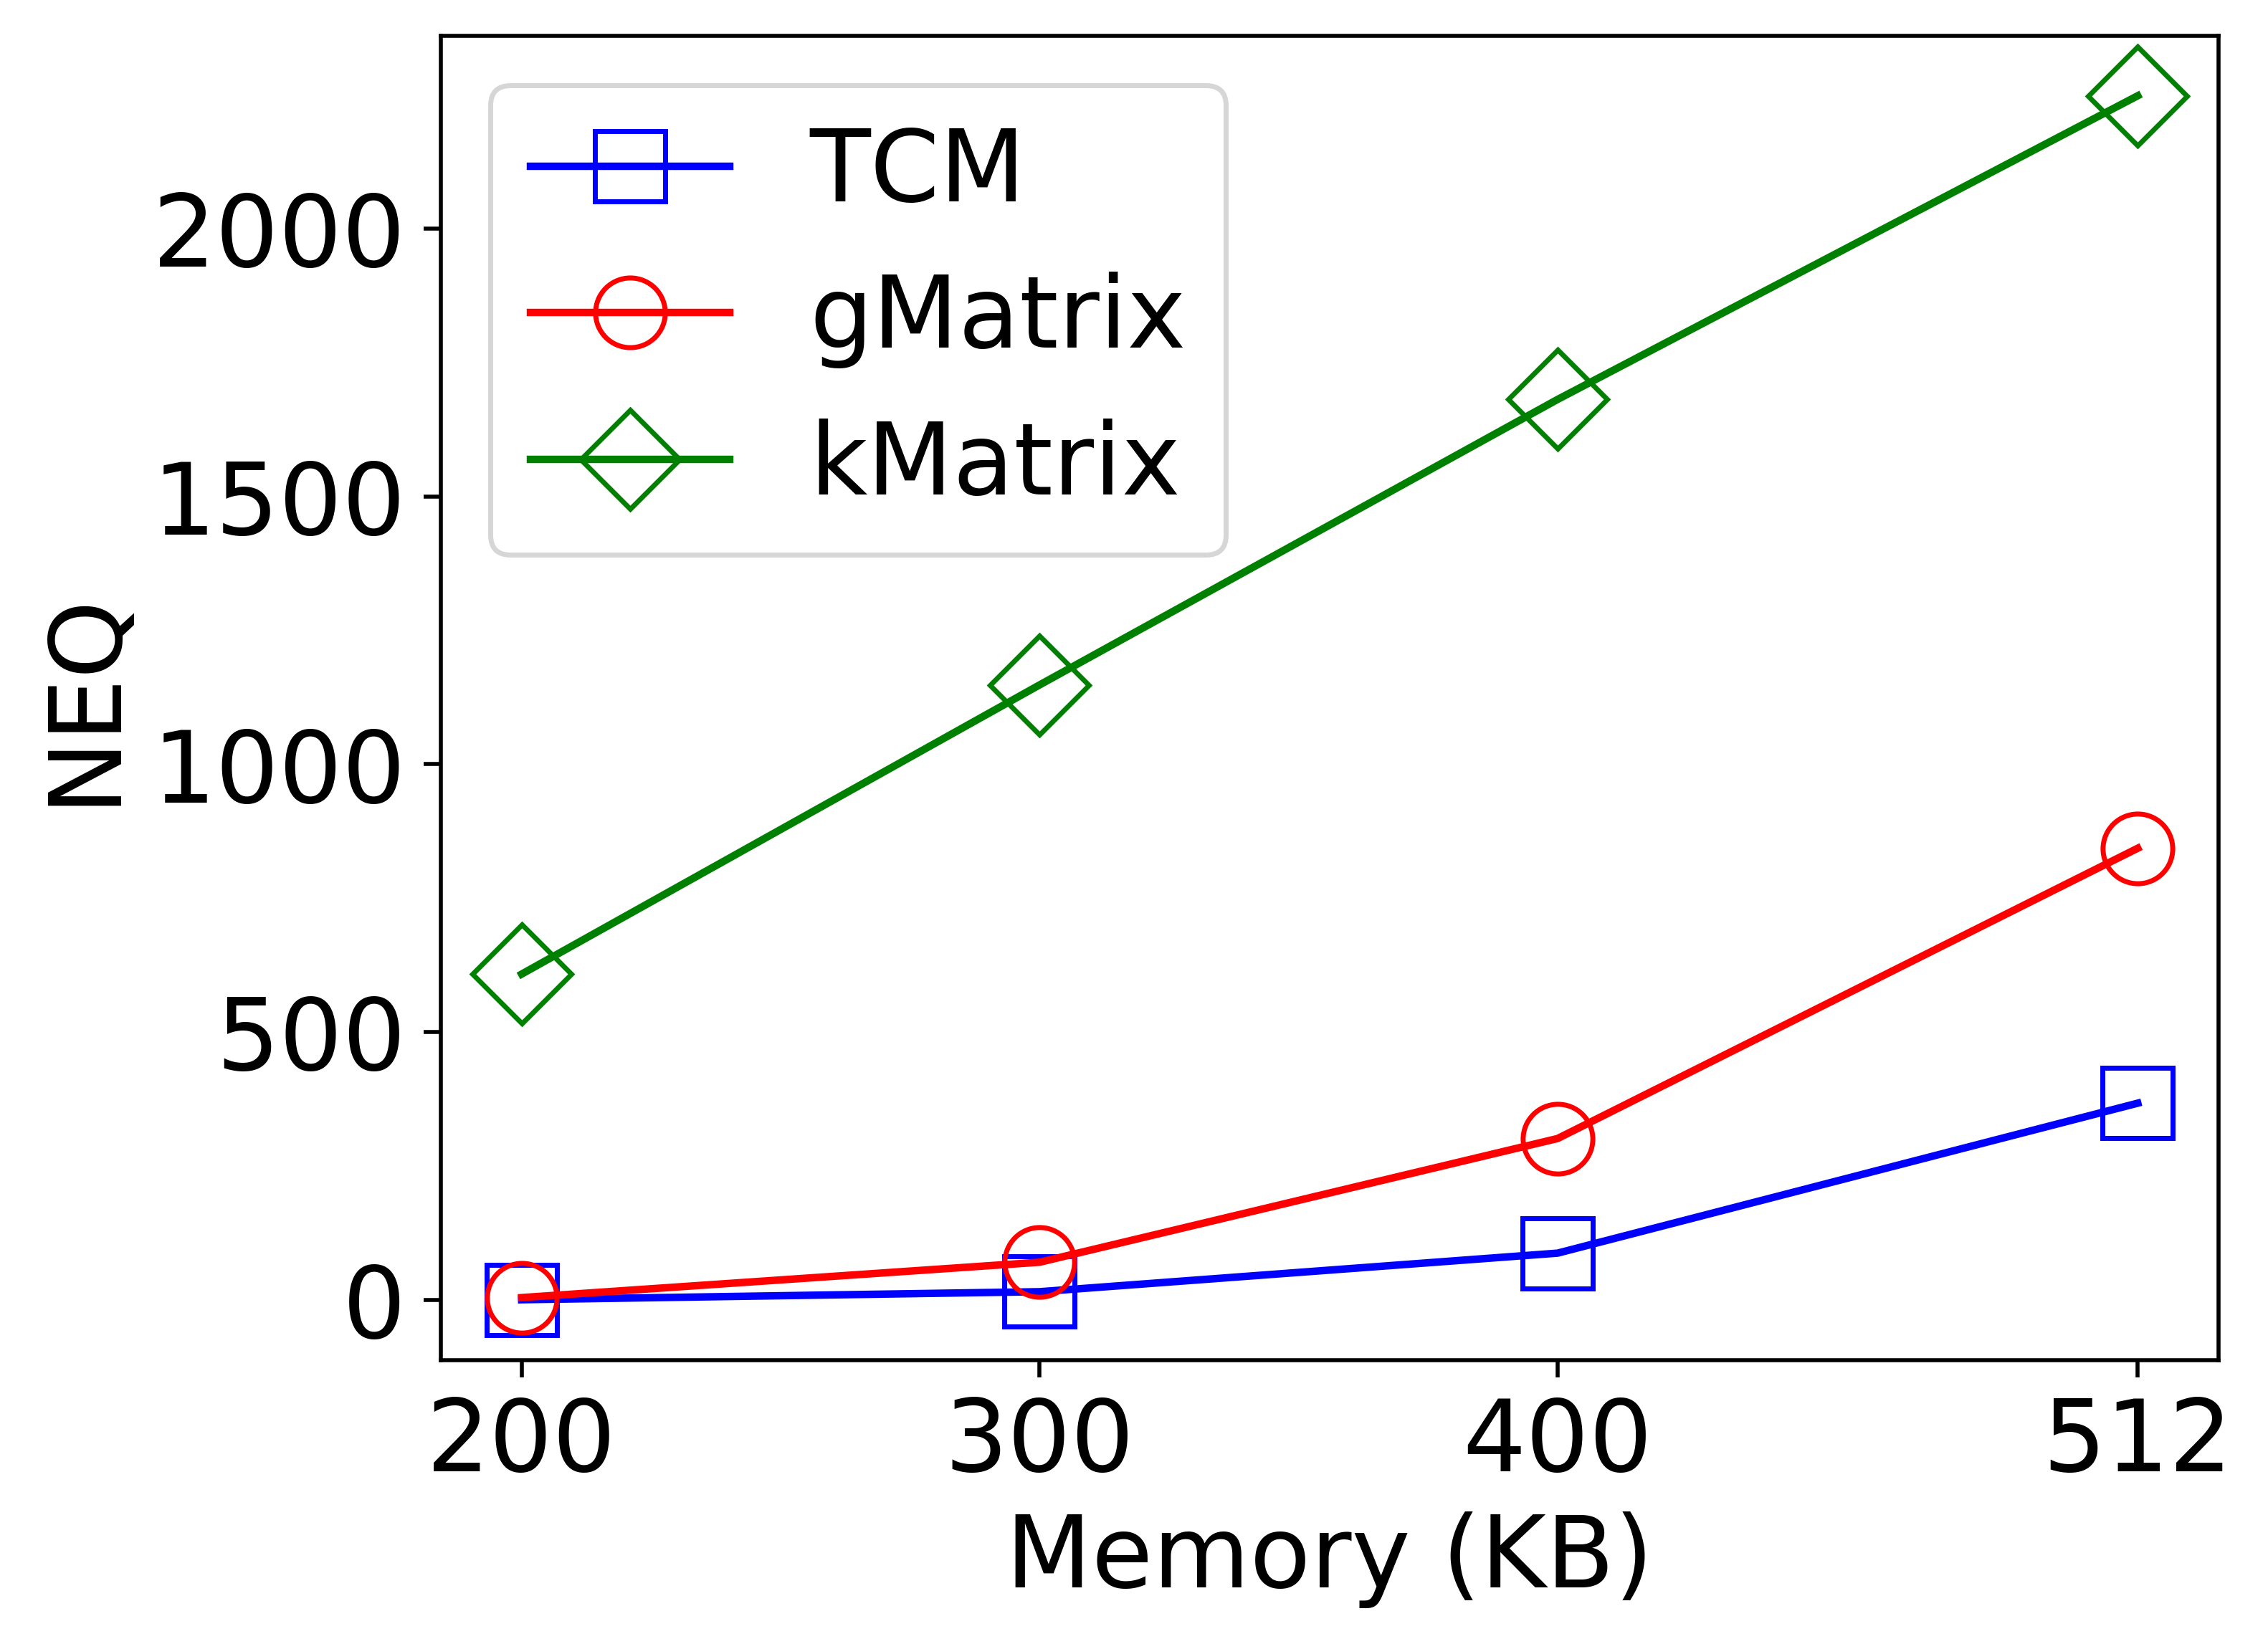
\includegraphics[width=0.45\linewidth]{img/edge_query_neq_unicorn-wget.png}}
    \hfill
    \subfloat[email-EuAll\label{fig:neq-b}]{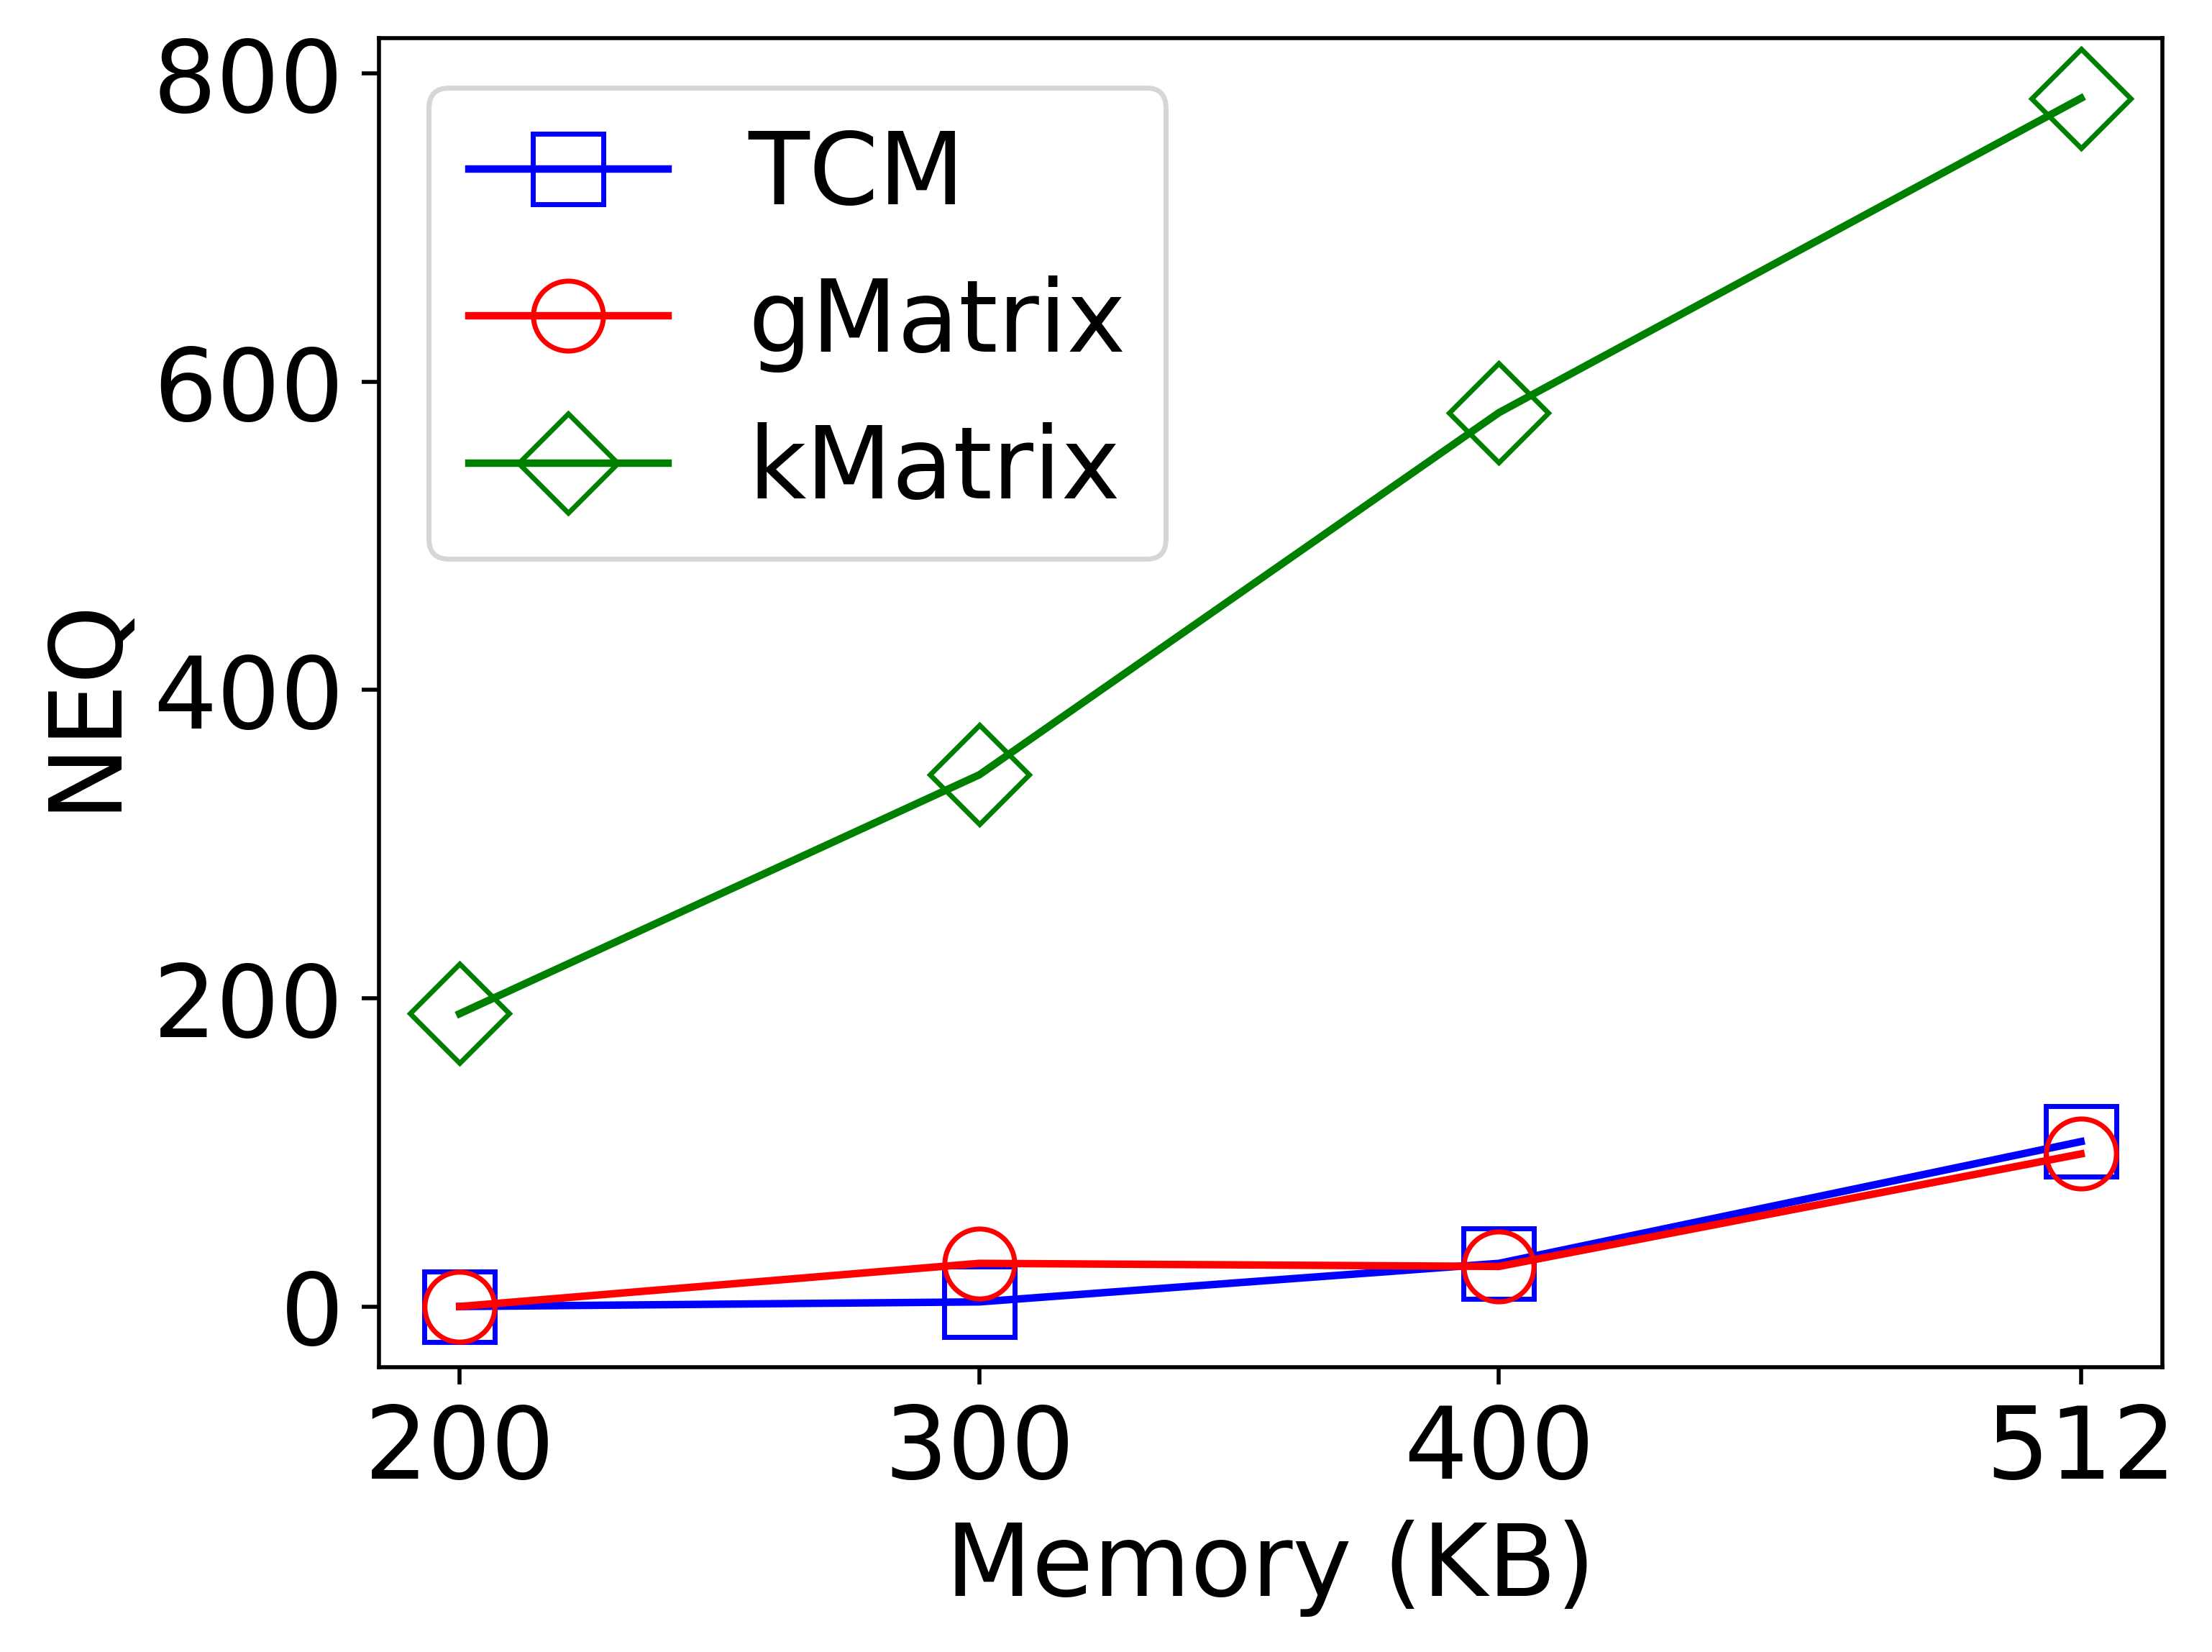
\includegraphics[width=0.45\linewidth]{img/edge_query_neq_email-EuAll.png}}
    \hfill
    \subfloat[cit-HepPh\label{fig:neq-c}]{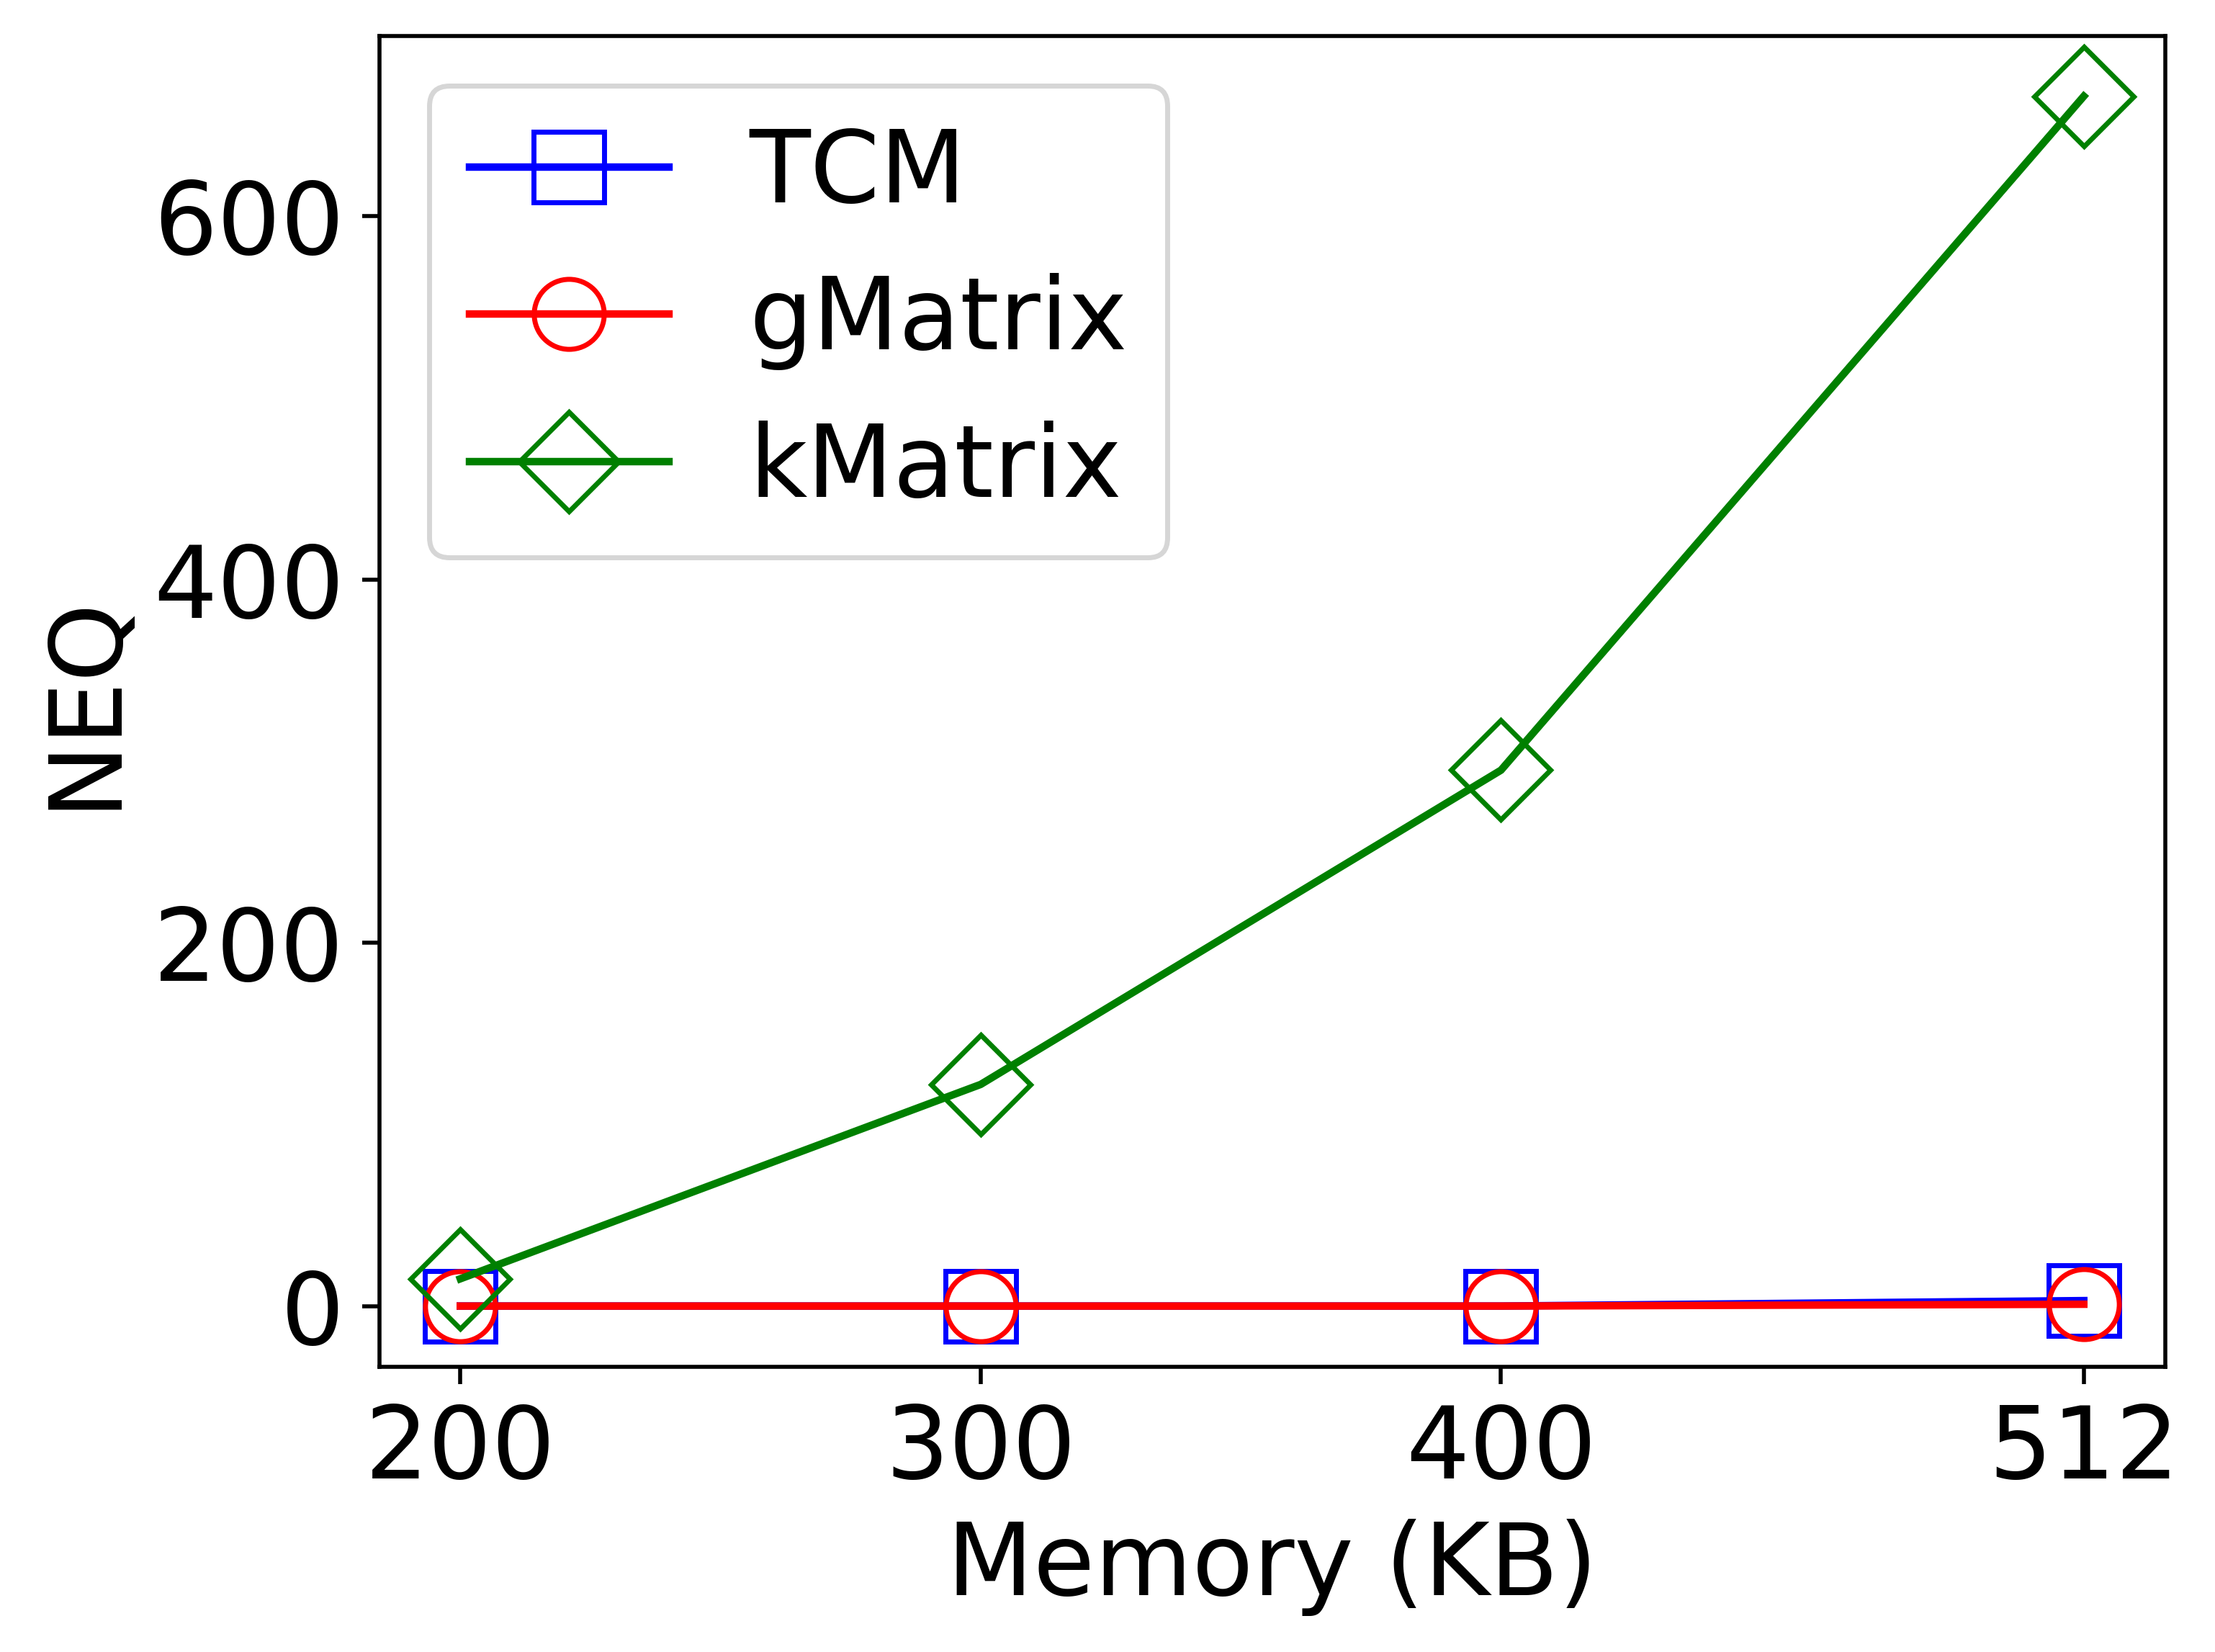
\includegraphics[width=0.45\linewidth]{img/edge_query_neq_cit-HepPh.png}}
    \caption{Number of effective queries}
    \label{fig:edgq-queries-neq-test}
\end{figure}

The number of effective queries for each sketch was calculated by querying the sketches against 10,000 edges chosen through reservoir sampling from the original dataset. kMatrix has surpassed the accuracy of both TCM and gMatrix for all the scenarios that we have tested. The results for cit-HepPh in Fig.~\ref{fig:neq-c} shows that kMatrix has been able to effectively answer a significantly larger number of queries where the other sketches failed due to hash collisions. This is due to the sketch partitioning process where kMatrix try to minimize the hash collisions in contrast to TCM and gMatrix.  